\documentclass[11pt,a4paper,oneside]{article}
\usepackage{titlesec}
\usepackage{graphicx}
\usepackage{float}
\usepackage{xcolor}
\usepackage{indentfirst}
\usepackage{array}
\usepackage{setspace}
\usepackage{enumitem}
\usepackage[utf8]{inputenc}

\titleformat{\section}{\Large\bfseries}{\thesection}{1em}{}[{\titlerule[0.8pt]}]

\title{\textsc{Assignment - 1\\Operating System\\KCS-401}}
\author{Abhay Shanker Pathak\\United Institute of Technology, Prayagraj\\IT-Department}
\date{March 2020}

\begin{document}

\maketitle
\setlength{\parindent}{1cm}

\renewcommand{\abstractname}{About}
\begin{abstract}
	\centering
	\large{This assignment contains questions and thier solutions\\
	All the questions are categorized sectionwise}
\end{abstract}

\pagenumbering{roman}
\tableofcontents
\listoftables
\listoffigures
\clearpage

\pagenumbering{arabic}

\section{Question}
\bgroup \bfseries
\noindent Consider the following snapshot at time T0 of the system and answer the following questions using Banker's algorithm
\begin{enumerate}
		\item Compute the total number of resource of each type.
		\item Compute the need matrix
		\item Is the system in a safe mode?
		\item If a request from P1 arrives for (0, 4, 2, 0), can the request granted immediately?
\end{enumerate}
\egroup{}

\begin{center}
	% this table centering{above} isn't working
	\begin{table}[h]
		\begin{tabular}{ ||>{\bfseries} m{7em} || m{7em} || m{7em} || m{7em} ||}
			\hline
			& \textbf{Allocation} & \textbf{Max} & \textbf{Available} \\
			\hline
			& a b c d & a b c d & a b c d \\
			\hline
			P0 & 0 0 1 2 & 0 0 1 2 & 1 5 2 0 \\
			\hline
			P1 & 1 0 0 0 & 1 7 5 0 & \\
			\hline
			P2 & 1 3 5 4 & 2 3 5 6 & \\
			\hline
			P3 & 0 6 3 2 & 0 6 5 2 & \\
			\hline
			P4 & 0 0 1 4 & 0 6 5 6 & \\
			\hline
		\end{tabular}
		\caption{data table, banker's algorithm}
	\end{table}
\end{center}

\begin{figure}[hbt!]
	\centering
	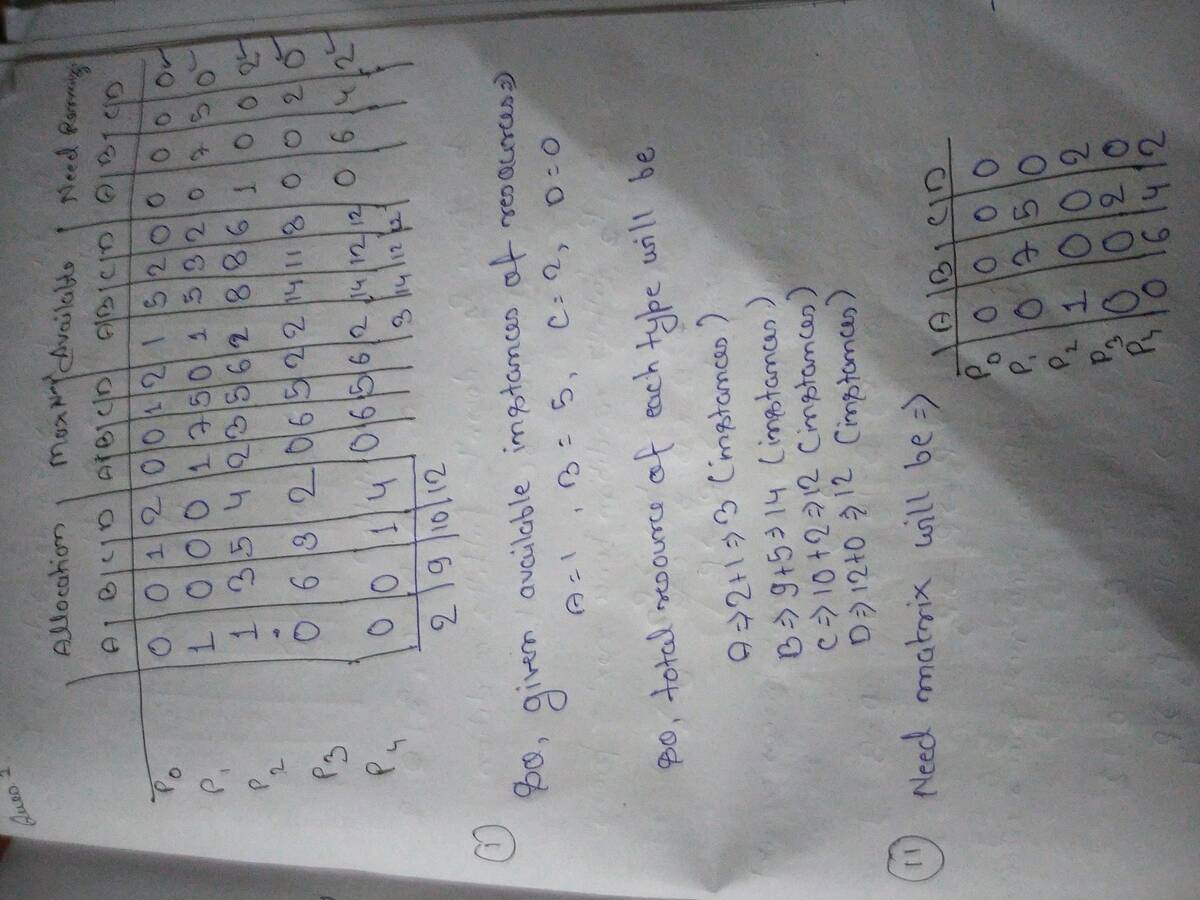
\includegraphics[width=0.6\textwidth, angle=-90]{images/red_images/q1i1.jpg}
	\caption{page 1 of solution for ques 1}
\end{figure}

\begin{figure}[hbt!]
	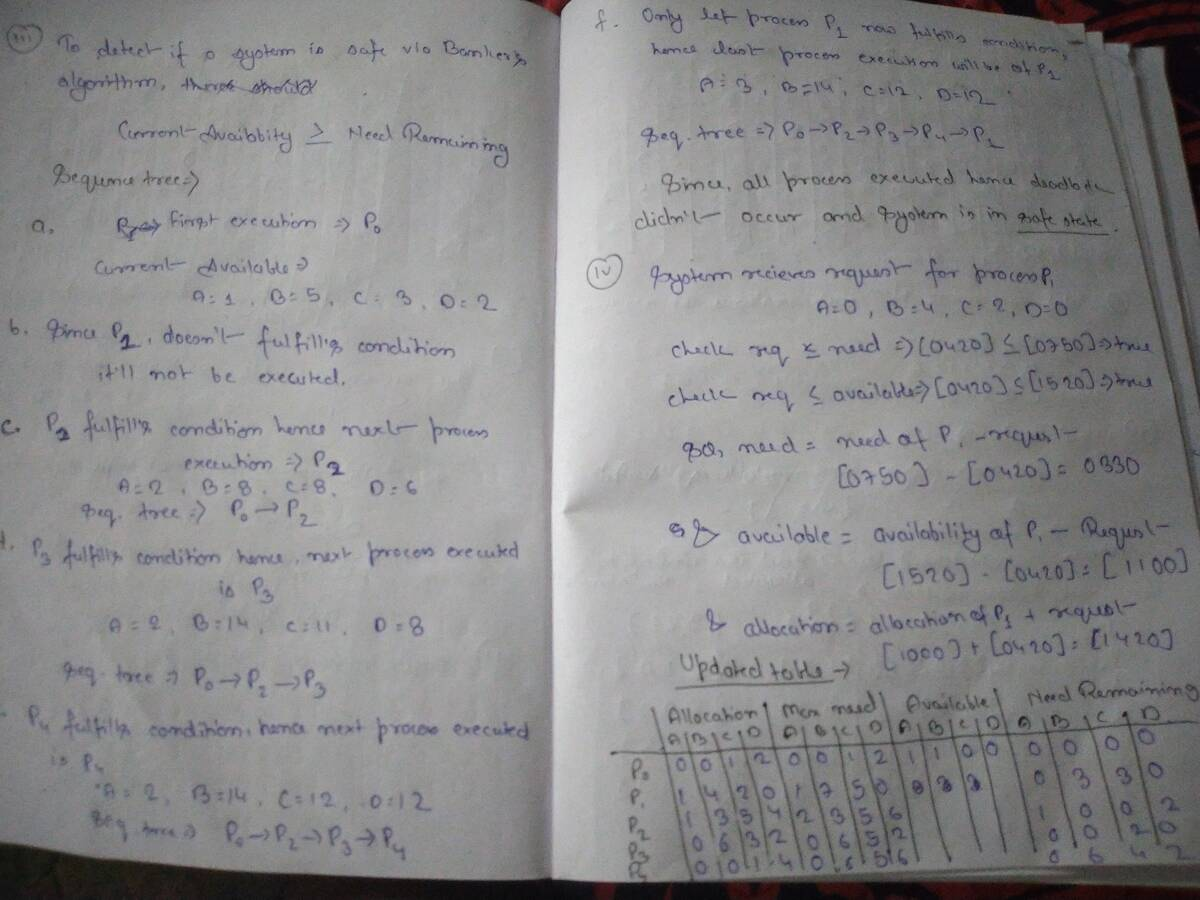
\includegraphics[width=1\textwidth]{images/red_images/q1i2.jpg}
	\caption{page 2 of solution for ques 1}
\end{figure}


\clearpage

\section{Question}
\bgroup \bfseries
\noindent Consider the set of process given in the table and draw the \textcolor{blue}{Gantt Chart} for \underline{preemptive} cases and find out the average waiting time, average turnaround time, throughput and CPU utilization for following scheduling algorithm.\\
Note: Larger priority number has higher priority

\begin{enumerate}[label=\alph*]
		\item Round Robin
		\item SRT
		\item Priority
\end{enumerate}
\egroup{}

\begin{center}
	\begin{table}[h]
		\begin{tabular}{ ||>{\bfseries} m{7em} || m{7em} || m{7em} || m{7em} ||}
			\hline
			Process ID & \bfseries{Arrival time} & \bfseries{Execution time} & \textbf{Priority} \\
			\hline
			P0 & 0 & 5 & 4 \\
			\hline
			P1 & 2 & 4 & 2 \\
			\hline
			P2 & 2 & 2 & 6 \\
			\hline
			P3 & 4 & 4 & 3 \\
			\hline
		\end{tabular}
		\caption{Details to process}
	\end{table}
\end{center}

\begin{figure}[hbt!]
	\centering
	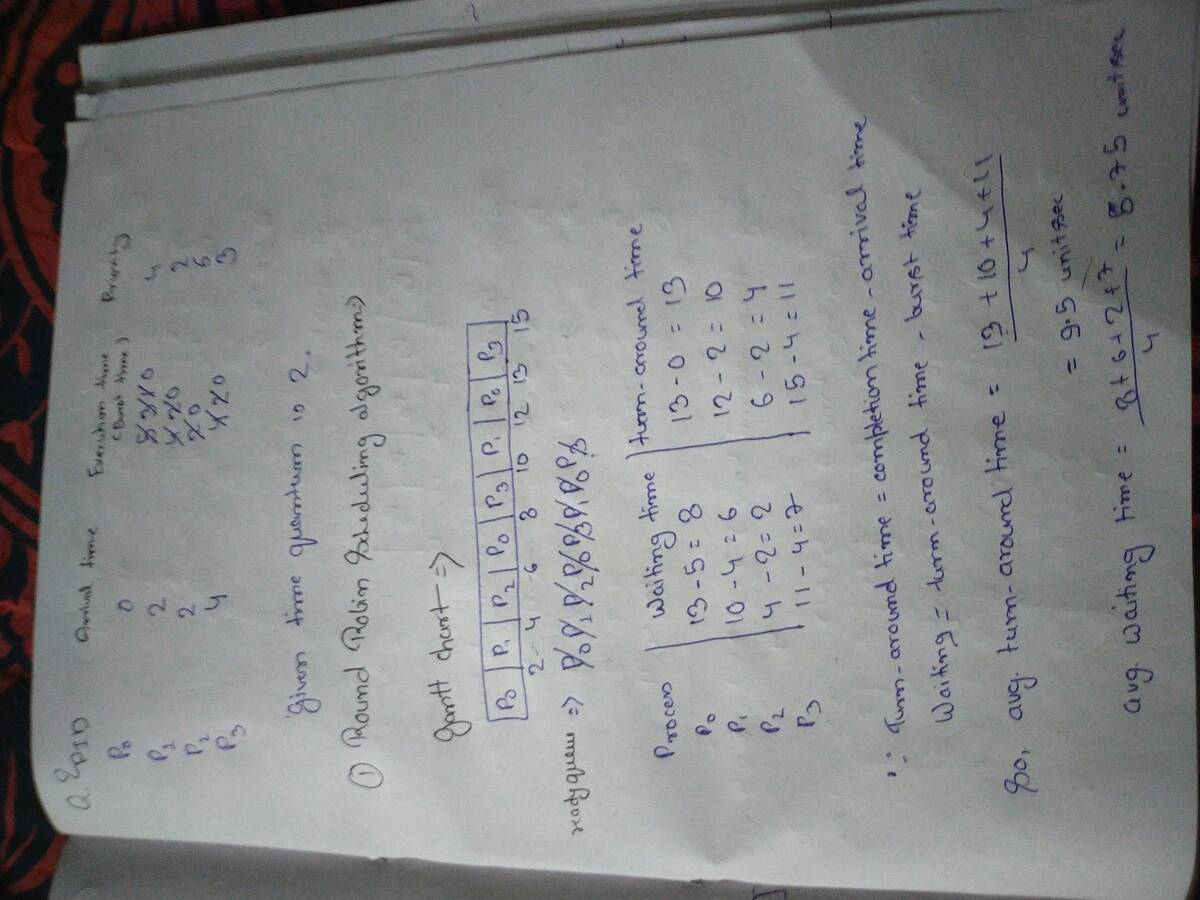
\includegraphics[width=0.6\textwidth, angle=-90]{images/red_images/q2i1.jpg}
	\caption{page 1 of solution for ques 2}
\end{figure}

\begin{figure}[hbt!]
	\centering
	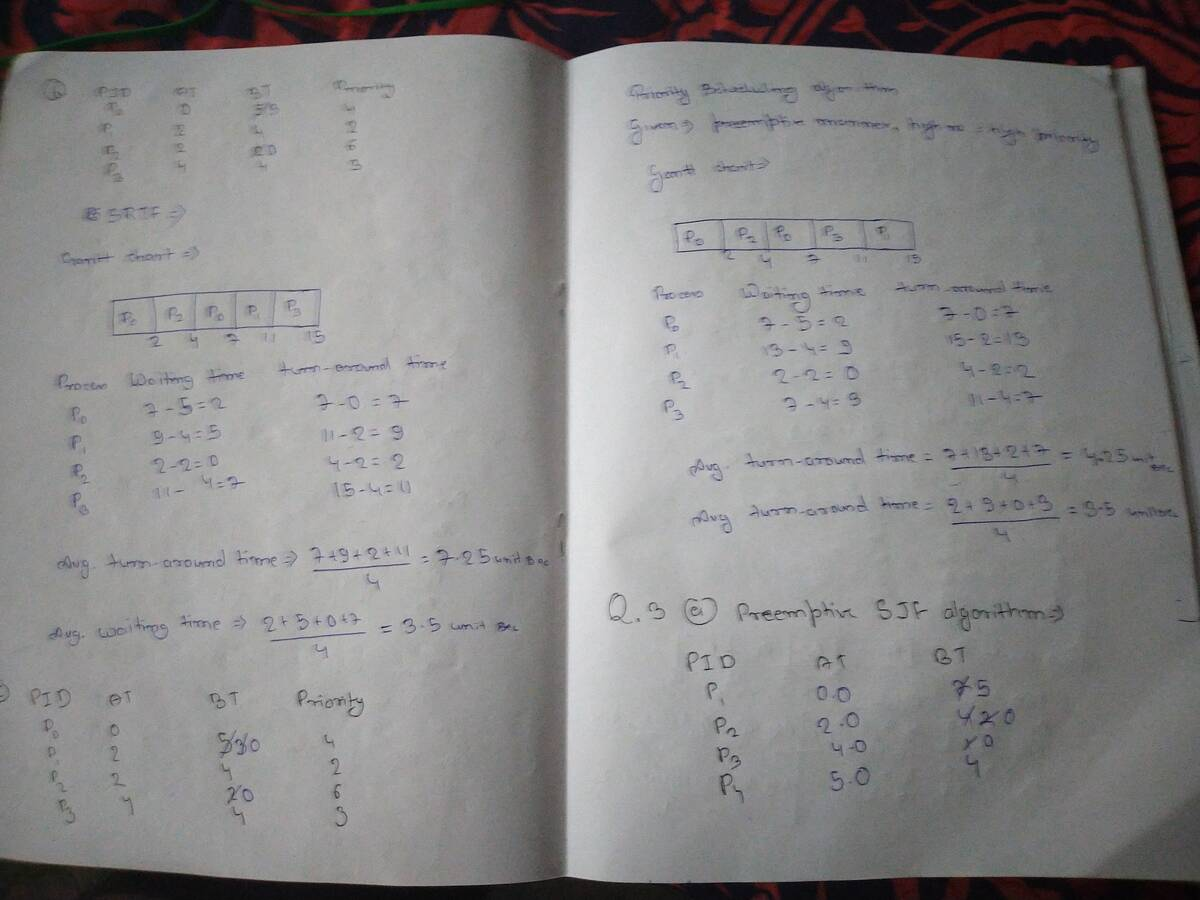
\includegraphics[width=1\textwidth]{images/red_images/q2i2.jpg}
	\caption{page 2 of solution for ques 2}
\end{figure}

\clearpage

\section{Question}

\bgroup \bfseries
\noindent Consider \underline{Non-preemptive} and \underline{preemptive} SJF algorithm; find out average waiting time in both.
\egroup{}

\begin{center}
	\begin{table}[h]
		\begin{tabular}{ ||>{\bfseries} m{7em} || m{10em} || m{12em} ||}
			\hline
			Process ID & \textbf{Arrival Time} & \textbf{Burst Time} \\
			\hline
			P1 & 0.0 & 7 \\
			\hline
			P2 & 2.0 & 4 \\
			\hline
			P3 & 4.0 & 1 \\
			\hline
			P4 & 5.0 & 4 \\
			\hline
		\end{tabular}
		\caption{Data to solve}
	\end{table}
\end{center}

\begin{figure}[hbt!]
	\centering
	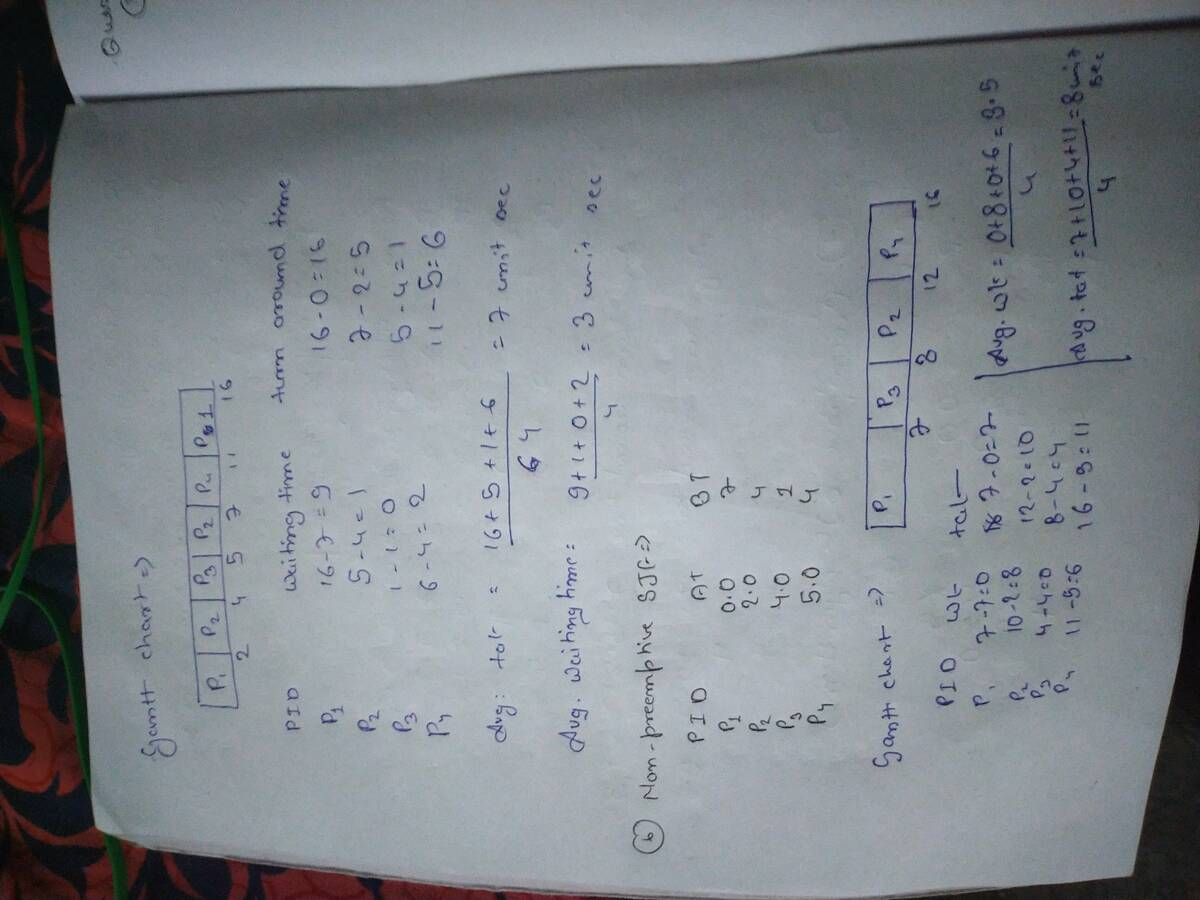
\includegraphics[width=1\textwidth, angle=-90]{images/red_images/q3i1.jpg}
	\caption{page 1 of solution for ques 3}
\end{figure}

\clearpage

\section{Question}

\bgroup \bfseries
\noindent Consider the following set of processes:
\egroup{}

\begin{center}
	\begin{table}[h]
		\begin{tabular}{ ||>{\bfseries} m{7em} || m{7em} || m{7em} || m{7em} ||}
			\hline
			Process ID & \textbf{Arrival Time} & \textbf{Burst Time} & \textbf{Priority} \\
			\hline
			P1 & 0  & 6 & 3 \\
			\hline
			P2 & 1 & 4 & 1 \\
			\hline
			P3 & 2 & 5 & 2 \\
			\hline
			P4 & 3 & 8 & 4 \\
			\hline
		\end{tabular}
	\caption{Data chart to process}
	\end{table}
\end{center}

\bgroup \bfseries
\begin{enumerate}[label=(\roman*)]
		\item Draw the \textcolor{blue}{Gantt charts} and find the average waiting time and average turnaround time using SRTF, Round robin(time quantum=3) and preemptive priority scheduling.
		\item If the schedulers takes 0.2 unit of CPU time in Context Switching, calculate the percentage of CPU time wasted in each case.
\end{enumerate}
\egroup{}

\begin{figure}[hbt!]
	\centering
	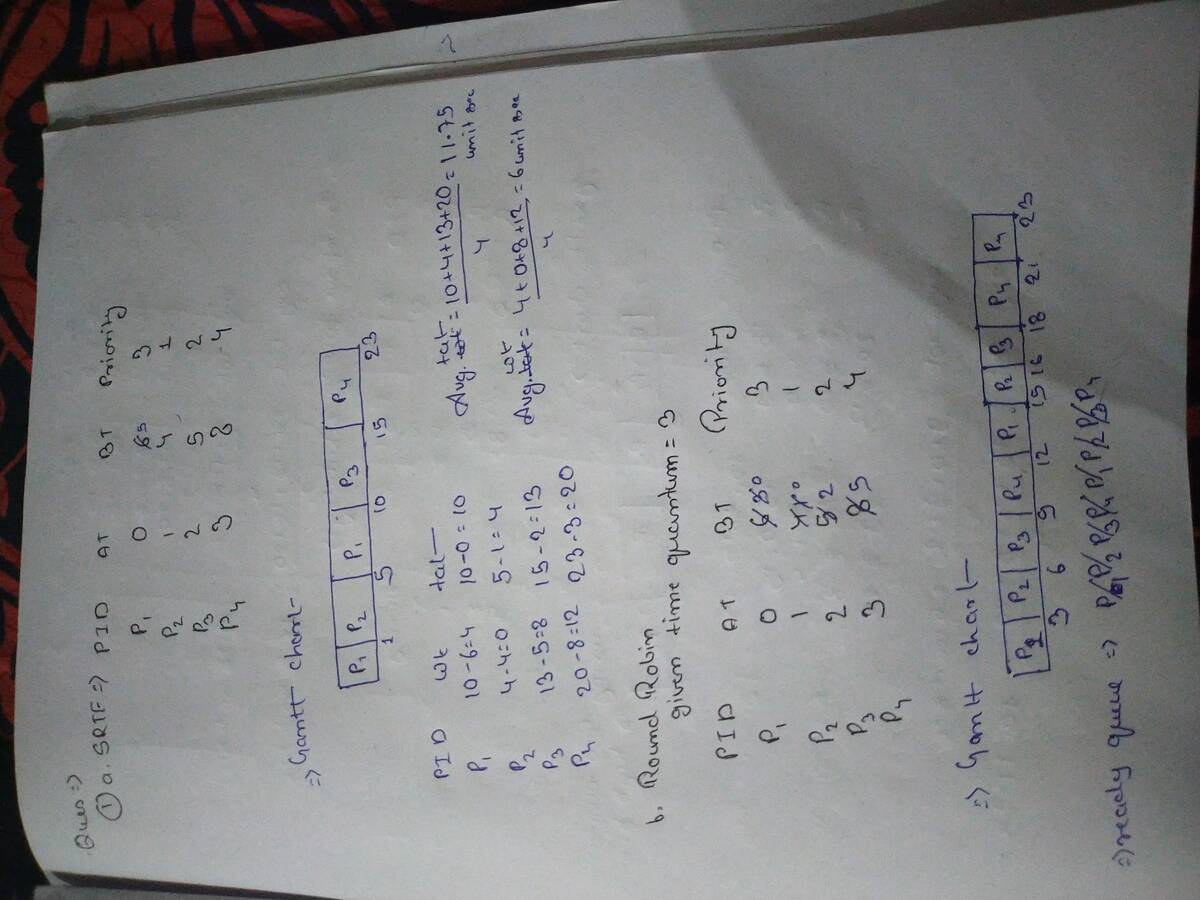
\includegraphics[width=0.7\textwidth, angle=-90]{images/red_images/q4i1.jpg}
	\caption{page 1 of solution for ques 4}
\end{figure}

\begin{figure}[hbt!]
	\centering
	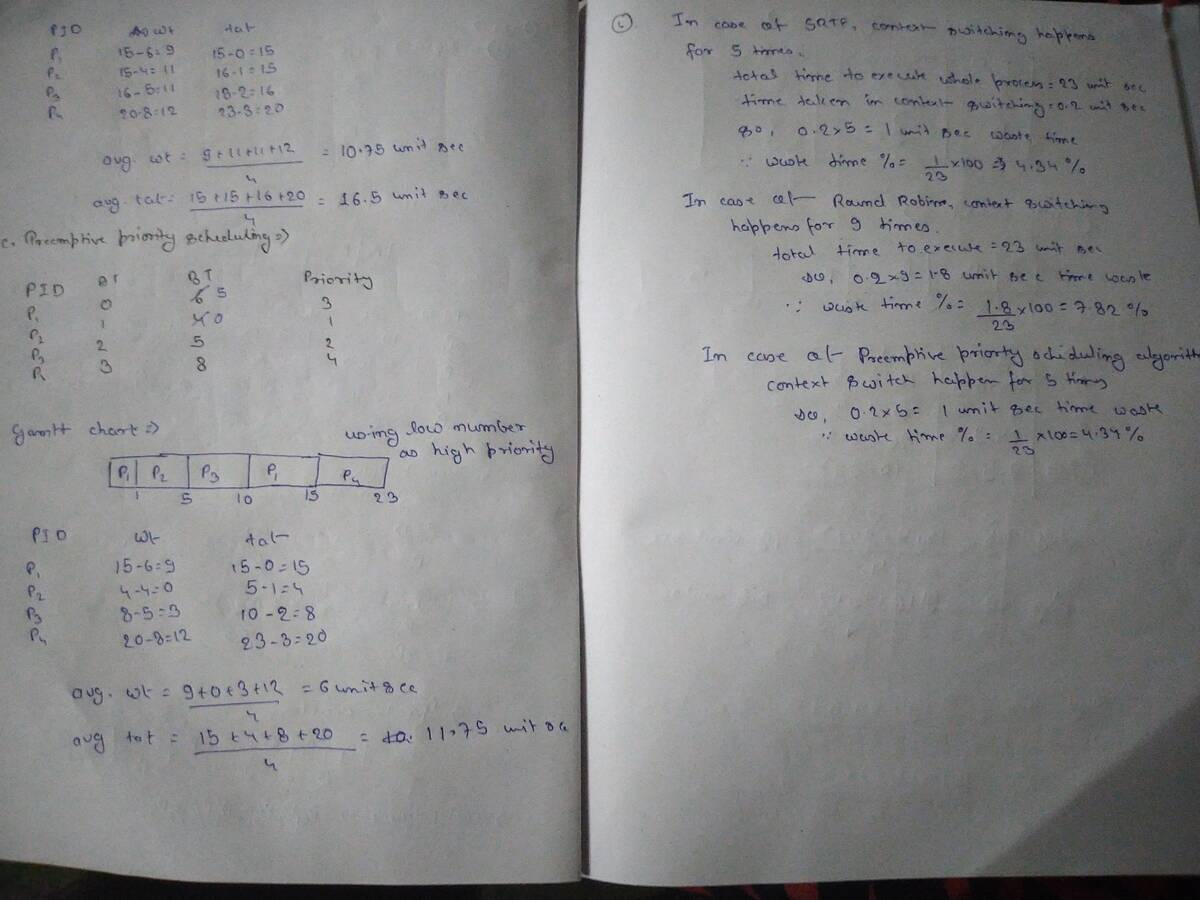
\includegraphics[width=1\textwidth]{images/red_images/q4i2.jpg}
	\caption{page 2 of solution for ques 4}
\end{figure}

\clearpage

\section{Question}
\bgroup \bfseries
\noindent Consider following set of process, CPU burst time and Arrival time given below:
\egroup{}

\begin{center}
	\begin{table}[h]
		\begin{tabular}{ ||>{\bfseries} m{7em} || m{10em} || m{12em} ||}
			\hline
			Process ID & \textbf{Arrival Time} & \textbf{Burst Time} \\
			\hline
			P1 & 8 & 0 \\
			\hline
			P2 & 4 & 1 \\
			\hline
			P3 & 9 & 2 \\
			\hline
			P4 & 5 & 3 \\
			\hline
		\end{tabular}
		\caption{Provided Data to solve}
	\end{table}
\end{center}

\bgroup \bfseries
Draw the \textcolor{blue}{Gantt charts} and find the average waiting time and average turnaround time using SRTF CPU scheduling algorithm.
\egroup{}

\begin{figure}[hbt!]
	\centering
	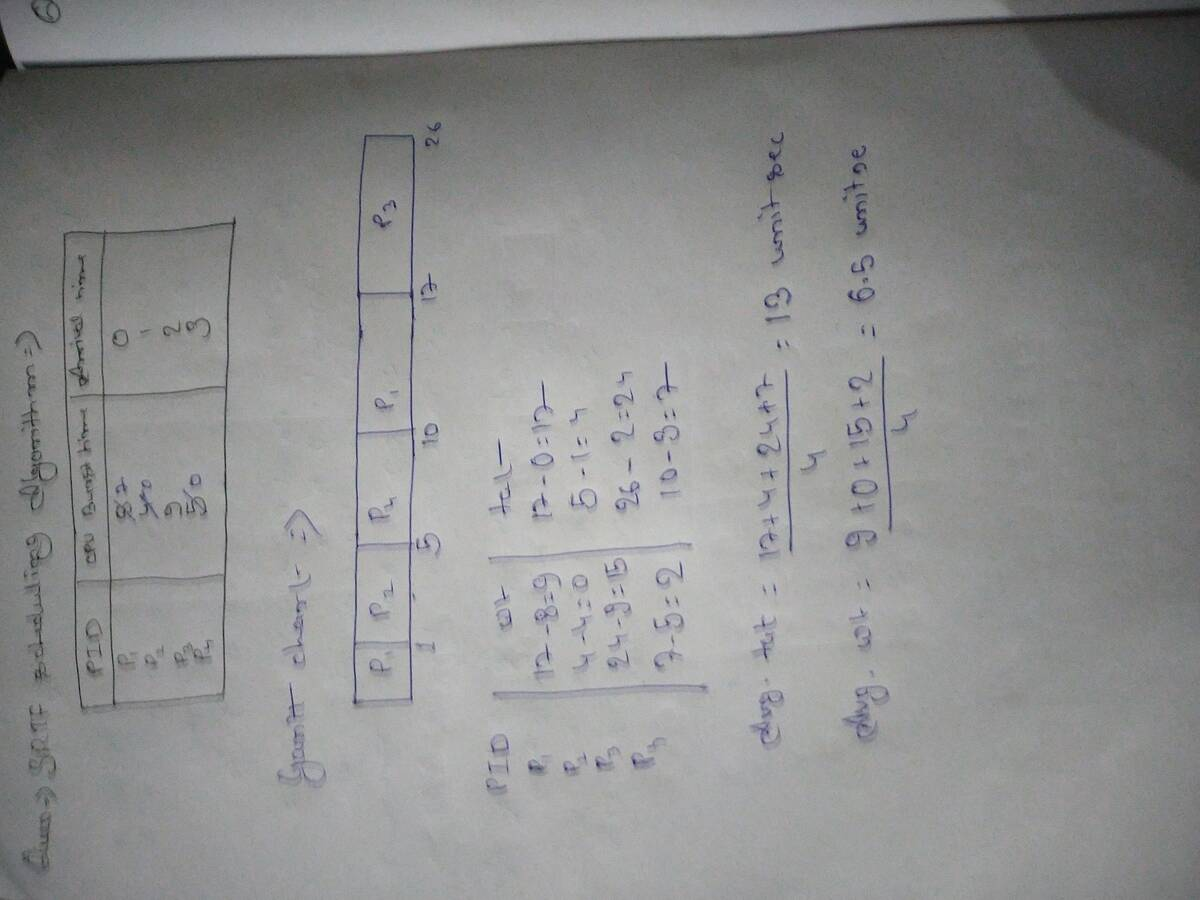
\includegraphics[width=0.9\textwidth, angle=-90]{images/red_images/q5i1.jpg}
	\caption{page 1 of solution for ques 5}
\end{figure}

\clearpage

\section{Question}

\bgroup \bfseries
\noindent List various performance criteria for scheduling algorithms. Five process A, B, C, D and E require CPU burst 3, 5, 2, 5 and 5 units respectively. Their arrival times in the system are 0, 1, 3, 9 and 12 respectively. Draw \textcolor{blue}{Gantt chart} and compute the average turnaround time and average waiting time of these processes for the Shortest Job First(SJF) and Shortest Remaining Time First(SRTF).
\egroup{}

\vskip 1cm

There are several different criteria to consider when trying to select the ``best'' scheduling algorithm for a particular situation and environment, including:

\subsubsection{CPU utilization - }
Ideally the CPU woulb be busy 100\% of the time, so as to waste 0 CPU cycles. On a real system CPU usage should range from 40\% (lightly load) to 90 \% ( heavily loaded. )

\subsubsection{Throughput - }
Number of process completed per unit time. May range from 10 per second to 1 hour depending on the specific processes.

\subsubsection{Turnaround time - }
Time required for a particular process to complete, from submission time to completion. (Wall clock time.)

\subsubsection{Waiting time - }
How much time processes spen in the ready queue waiting their turn to get on the CPU.

\subsubsection{Load average - }
The average number of processes sitting in the ready queue waiting their turn to get into the CPU. Reported in 1-minute, 5-minute, and 15-minute averages(number aren't unique) by ``uptime'' and ``who''.

\subsubsection{Response time - }
The time taken in an interactive program from the issuance of a command to the \emph{commence} of a response to that command.

\vskip 1cm

In general one wants to optimize the average value of a criteria ( Maximize CPU utilization and throughput, and minimize all the others. ) However some times one wants to do something different, such as to minimize the maximum response time.

Sometimes it is most desirable to minimize the \textmd{variance} of a criteria than the actual value, i.e., users are more accepting of a consistent predictable system than an inconsistent one, even if it is a little bit slower.

\vskip 1cm

\begin{figure}[hbt!]
	\centering
	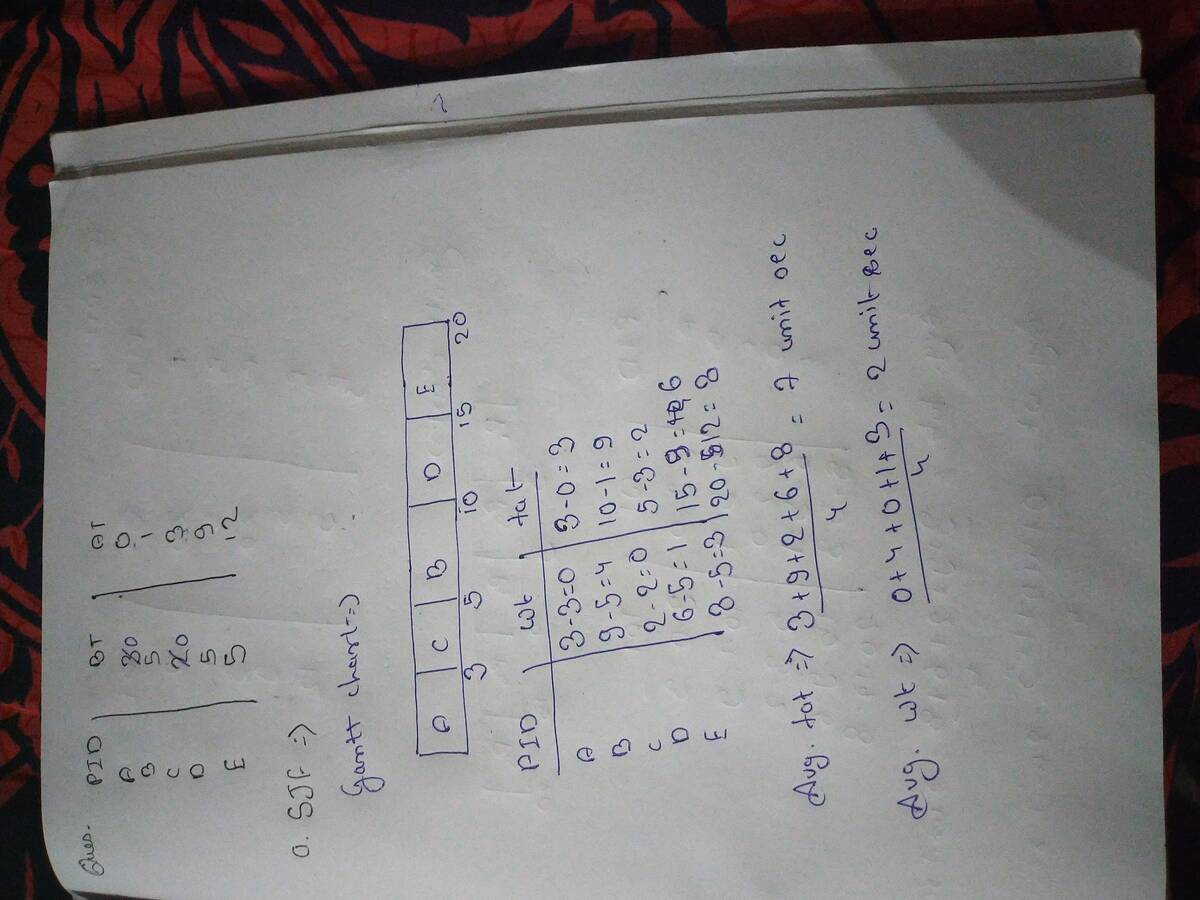
\includegraphics[width=1\textwidth, angle=-90]{images/red_images/q6i1.jpg}
	\caption{page 1 of solution for ques 6}
\end{figure}

\begin{figure}[hbt!]
	\centering
	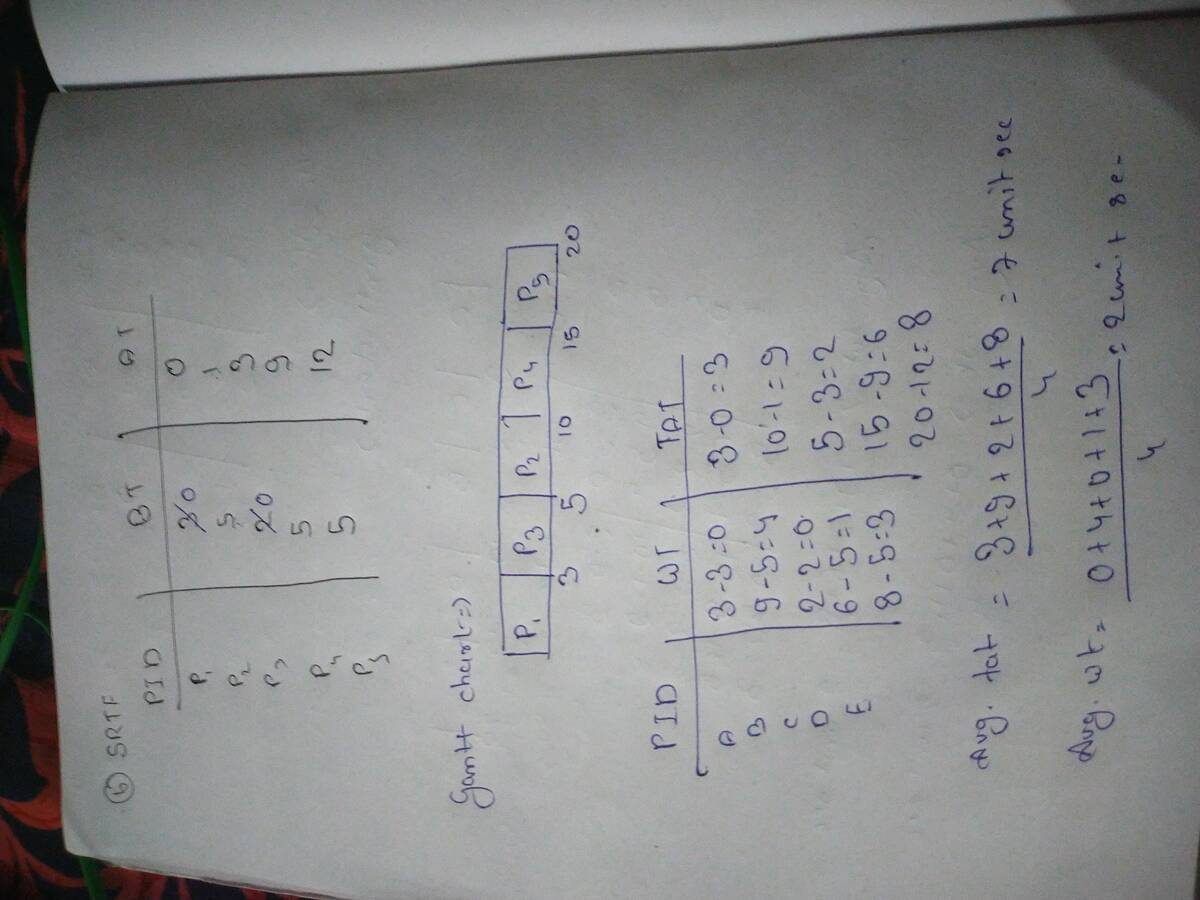
\includegraphics[width=1.2\textwidth, angle=-90]{images/red_images/q6i2.jpg}
	\caption{page 2 of solution for ques 6}
\end{figure}


\clearpage

\section{Question}

\bgroup \bfseries
\noindent Describe the banker's algorithm for safe allocation. Consider a system with five process and three resource types and at time 'T' the following snapshot of the system has been taken:
\egroup{}

% \begin{center}
% 	\begin{table}[h]
% 		\begin{tabular}{ ||>{\bfseries} l || @{}l@{} || @{}l@{} || @{}l@{} ||}
% 			\hline
% 			& \textbf{Allocated} & \textbf{Maximum} & \textbf{Available} \\
% 			\hline
% 			PID &
% 			\begin{tabular}{ c | c | c }
% 				R1 & R2 & R3 \\
% 			\end{tabular} &
% 			\begin{tabular}{ c | c | c }
% 				R1 & R2 & R3 \\
% 			\end{tabular} &
% 			\begin{tabular}{ c | c | c }
% 				R1 & R2 & R3 \\
% 			\end{tabular} \\
% 			\hline
% 			P1 &
% 			\begin{tabular}{ c | c | c }
% 				1 & 1  & 2 \\
% 			\end{tabular} &
% 			\begin{tabular}{ c | c | c }
% 				4 & 3 & 3 \\
% 			\end{tabular} &
% 			\begin{tabular}{ c | c | c }
% 				3 & 1 & 0 \\
% 			\end{tabular} \\
% 			\hline
% 			P2 &
% 			\begin{tabular}{ c | c | c }
% 				2 & 1 & 2 \\
% 			\end{tabular} &
% 			\begin{tabular}{ c | c | c }
% 				3 & 2 & 2 \\
% 			\end{tabular} & \\
% 			\hline
% 			P3 &
% 			\begin{tabular}{ c | c | c }
% 				4 & 0 & 1 \\
% 			\end{tabular} &
% 			\begin{tabular}{ c | c | c }
% 				9 & 0 & 2 \\
% 			\end{tabular} & \\
% 			\hline
% 			P4 &
% 			\begin{tabular}{ c | c | c }
% 				0 & 2 & 0 \\
% 			\end{tabular} &
% 			\begin{tabular}{ c | c | c }
% 				7 & 5 & 3 \\
% 			\end{tabular} & \\
% 			\hline
% 			P5 &
% 			\begin{tabular}{ c | c | c }
% 				1 & 1 & 2 \\
% 			\end{tabular} &
% 			\begin{tabular}{ c | c | c }
% 				11 & 2 & 3 \\
% 			\end{tabular} & \\
% 			\hline
% 		\end{tabular}
% 		\caption{Data to solve with banker's algorithm}
% 	\end{table}
% \end{center}

\begin{table}[htpb!]
	\centering
	\begin{tabular}{ ||>{\bfseries} l || c | c | c || c | c | c || c | c | c ||}
		\cline{1-10}	% we could use \hline here, this is just to know
		& \multicolumn{3}{ | c || }{\textbf{Allocated}} & \multicolumn{3}{ | c || }{\textbf{Maximum}} & \multicolumn{3}{ | c || }{\textbf{Available}} \\
		\hline
		PID & R1 & R2 & R3 & R1 & R2 & R3 & R1 & R2 & R3 \\
		\hline
		P1 & 1 & 1 & 2 & 4 & 3 & 3 & 3 & 1 & 0 \\
		\hline
		P2 & 2 & 1 & 2 & 3 & 2 & 2 & & & \\
		\hline
		P3 & 4 & 0 & 1 & 9 & 0 & 2 & & & \\
		\hline
		P4 & 0 & 2 & 0 & 7 & 5 & 3 & & & \\
		\hline
		P5 & 1 & 1 & 2 & 11 & 2 & 3 & & & \\
		\hline
	\end{tabular}
	\caption{Data to solve with Banker's Algorithm}
\end{table}



\bgroup \bfseries
\begin{enumerate}[label=(\roman*)]
	\item Determine the total amount of resources of each type.
		\item Compute the need matrix.
			\item Determine the state is safe or not using Banker's algorithm.
				\item Would the following request be granted in the current state?
					\begin{enumerate}
							\item P1\textless3, 3, 1\textgreater
							\item P2\textless2, 1, 0\textgreater
					\end{enumerate}
\end{enumerate}
\egroup{}

\begin{figure}[hbt!]
	\centering
	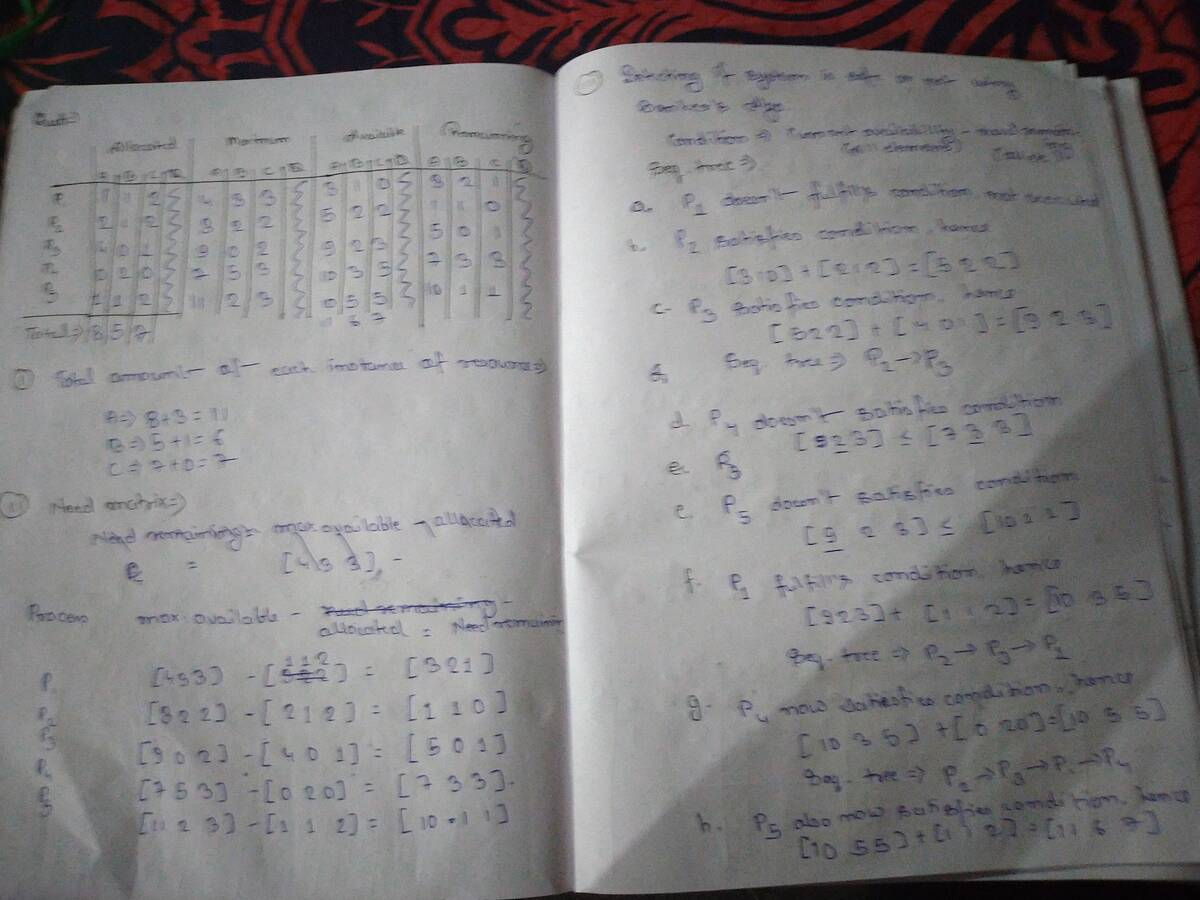
\includegraphics[width=1\textwidth]{images/red_images/q7i1.jpg}
	\caption{page 1 of solution for ques 7}
\end{figure}

\begin{figure}[hbt!]
	\centering
	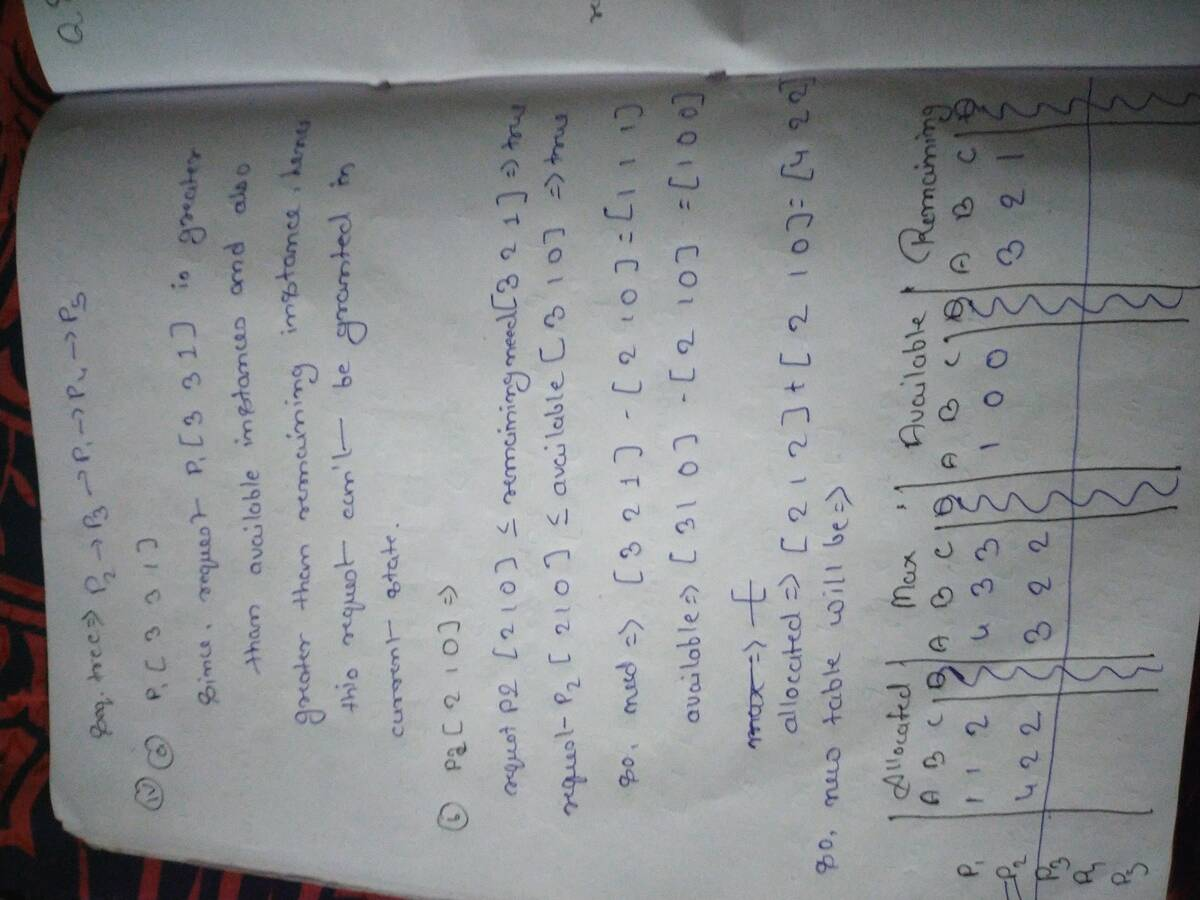
\includegraphics[width=1.5\textwidth, angle=-90]{images/red_images/q7i2.jpg}
	\caption{page 2 of solution for ques 7}
\end{figure}

\end{document}
